\section{Цель работы}
Освоение способа параметрического представления выходной переменной и вектора состояния линейной модели объекта.


\section{Теоретические сведения}
Параметризацией модели объекта называется представление его выходной переменной (или вектора состояния) в виде линейной регрессионной модели, т.е. в виде произведения вектора (матрицы) постоянных параметров и вектора (матрицы) известных функций:
\begin{equation}
    y = \theta^T \omega,
    \qquad
    \text{или}
    \qquad
    x = \!\!\! \sum_{i=1}^{n+m+1} \!\! \theta_i \xi_i,
\end{equation}
где $\theta$~--- вектор постоянных параметров, $\omega$~--- вектор известных функций, $\theta_i$~--- компоненты вектора постоянных параметров, $\xi_n \in \mathbb{R}^n$~--- измеряемые вектора.

\section{Исходные данные}
Варианту \textnumero2 соответствует следующий набор исходных данных:
\begin{equation}
    a_1 = 2,
    \quad
    a_0 = 1,
    \quad
    b_1 = 1,
    \quad
    b_0 = 3,
    \quad
    k_1 = \sqrt{0.02},
    \quad
    k_0 = 0.01,
    \quad
    u = \sin{t} + 0.5 \cos{2t}
\end{equation}


\section{Результаты расчетов и моделирования}
\subsection{Построение модели исходного объекта}
Модель рассматриваемого объекта в форме ВСВ:
\begin{align}
    & \dot{x} = Ax + bu, \label{eq_state_space_model_of_plant}\\
    & y = Cx,
\end{align}
где
\begin{equation}
    A =
    \begin{bmatrix}
        -a_1 & 1 \\
        -a_0 & 0
    \end{bmatrix}\!\!,
    \qquad
    b = 
    \begin{bmatrix}
        b_1 \\ b_0
    \end{bmatrix}\!\!,
    \qquad
    C =
    \begin{bmatrix}
        1 & 0
    \end{bmatrix}\!\!\ldotp
\end{equation}
Соответствующие ей начальные условия $\{x_1(0), x_2(0)\}$ связаны с начальными условиями $\{y(0), \dot{y}(0)\}$ следующими выражениями
\begin{align}
    & x_1(0) = y(0), \\
    \dot{x}_1(0) = \dot{y}(0) = -a_1 y(0) + x_2(0) + b_1 \underbrace{u(0)}_{=0}
    \quad \Rightarrow \quad
    & x_2(0) = \dot{y}(0) + a_1 y(0) 
\end{align}


\subsection{Параметризация относительно выходной переменной}
Модель рассматриваемого объекта в форме ВСВ:
\begin{equation}
    \ddot{y} + a_1 \dot{y} + a_0 y = b_1 \dot{u} + b_0 u
\end{equation}
После применения к правой и левой частям этого уравнения оператора
\begin{equation}
    H(s) = \frac{1}{K(s)},
\end{equation}
где $K(s) = s^2 + k_1 s + k_0$ и некоторого количества алгебраических преобразований достигается следующий результат:
\begin{gather}
    \frac{1}{K(s)}[\ddot{y} + a_1 \dot{y} + a_0 y] = \frac{1}{K(s)}[b_1 \dot{u} + b_0 u] \\
    %
    \frac{1}{K(s)}[\ddot{y}] + a_1 \frac{1}{K(s)}[\dot{y}] + a_0\frac{1}{K(s)}[y] = b_1 \frac{1}{K(s)}[\dot{u}] + b_0\frac{1}{K(s)}[u] \\
    %
    \frac{s^2}{K(s)}[y] + a_1 \frac{s}{K(s)}[y] + a_0\frac{1}{K(s)}[y] = b_1 \frac{s}{K(s)}[u] + b_0\frac{1}{K(s)}[u] \\
    %
    \frac{s^2 \pm (k_1 s + k_0)}{K(s)}[y] = -a_1 \frac{s}{K(s)}[y] - a_0\frac{1}{K(s)}[y] + b_1 \frac{s}{K(s)}[u] + b_0\frac{1}{K(s)}[u] \\
    %
    y = \frac{k_1 s + k_0}{K(s)}[y] -a_1 \frac{s}{K(s)}[y] - a_0\frac{1}{K(s)}[y] + b_1 \frac{s}{K(s)}[u] + b_0\frac{1}{K(s)}[u] \\
    %
    y = (k_1 - a_1) \underbrace{\frac{s}{K(s)}[y]}_{\xi_2} + (k_0 - a_0) \underbrace{\frac{1}{K(s)}[y]}_{\xi_1} + b_1 \underbrace{\frac{s}{K(s)}[u]}_{\nu_2} + b_0 \underbrace{\frac{1}{K(s)}[u]}_{\nu_1} \\
    %
    y = \theta^T \omega,
\end{gather}
где
\begin{equation}
    \theta^T =
    \begin{bmatrix}
        k_1 - a_1 & k_0 - a_0 & b_1 & b_0
    \end{bmatrix}\!\!,
    \qquad
    \omega^T =
    \begin{bmatrix}
        \xi_2 & \xi_1 & \nu_2 & \nu_1
    \end{bmatrix}
\end{equation}

Схема моделирования, проверяющая работоспособность полученной регрессионной модели, и результаты ее запуска показаны на рисунках~\ref{img_for_output} и~\ref{img_output_graphs}.

\begin{figure}[p]
    \centering
    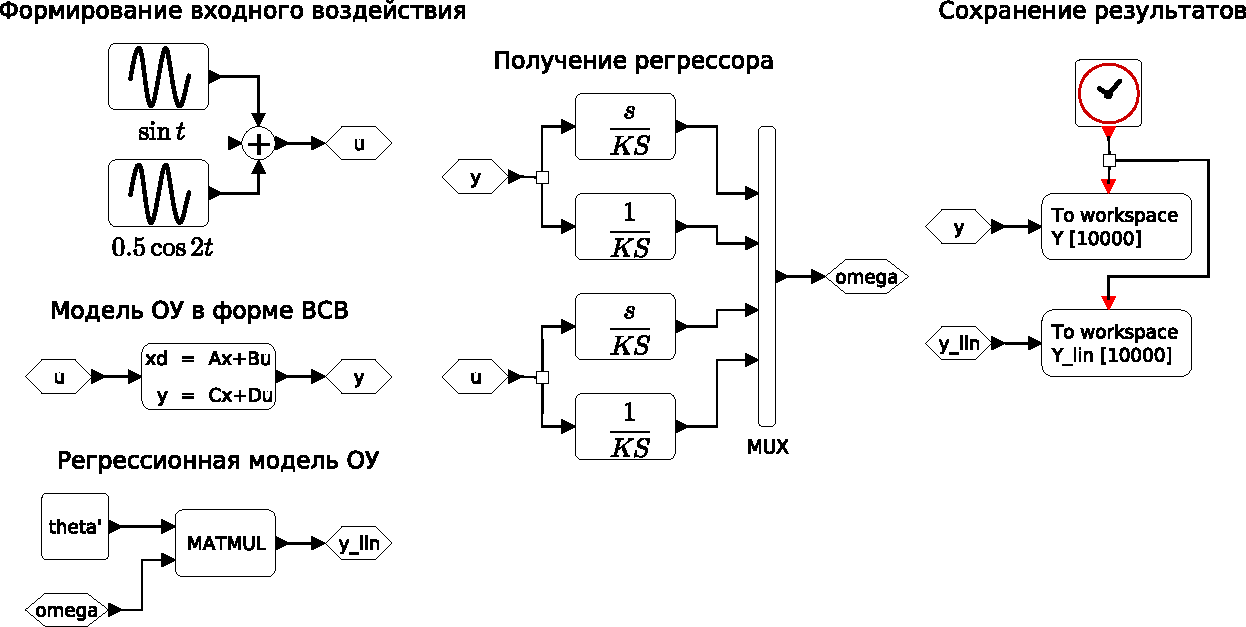
\includegraphics[width=\textwidth]{for_output.pdf}
    \caption{Схема моделирования, применяемая для проверки работы регрессионной модели.}
    \label{img_for_output}
\end{figure}

\begin{figure}[p]
    \centering
    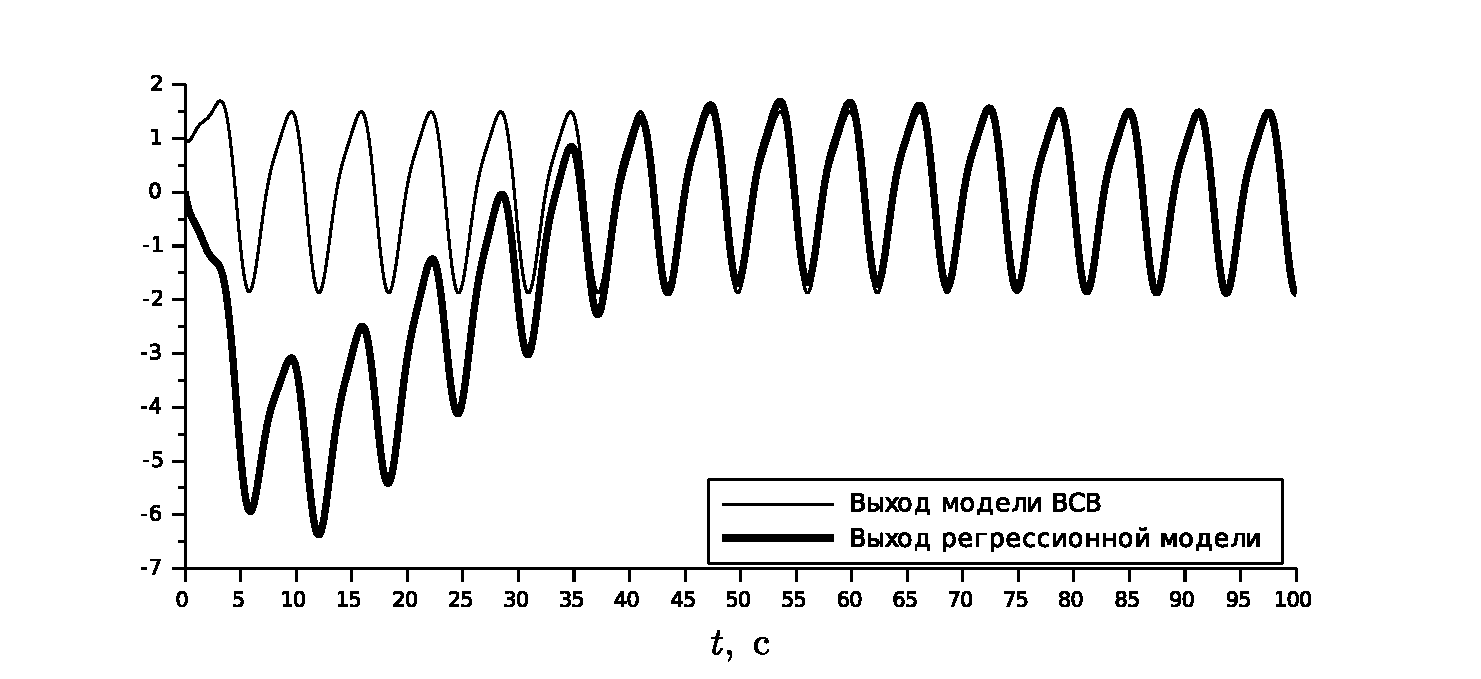
\includegraphics[width=1.05\textwidth]{output_graphs.pdf}
    \caption{Графики выходных сигналов моделей ОУ при $y(0)=1$ и $\dot{y}(0)=-1$.}
    \label{img_output_graphs}
\end{figure}


\newpage
\subsection{Параметризация относительно вектора состояния}
После применения к уравнению~\eqref{eq_state_space_model_of_plant} матричной передаточной функции
\begin{equation}
    \Phi(s) = (sI - A_0)^{-1},
\end{equation}
где
\begin{equation}
    A_0 =
    \begin{bmatrix}
        -k_1 & 1 \\
        -k_0 & 0
    \end{bmatrix} \!\!,
\end{equation}
достигается следующий результат:
\begin{gather}
    \Phi(s) [\dot{x}] = \Phi(s) A [x] + \Phi(s) b [u], \\
    %
    \Phi(s) (sI \pm A_0) [x] = \Phi(s) A [x] + \Phi(s) b [u], \\ 
    %
    x = \Phi(s) (A - A_0) [x] + \Phi(s) b [u], \\
    %
    x = \Phi(s) 
    \begin{bmatrix}
        k_1 - a_1 \\ k_0 - a_0        
    \end{bmatrix}
    [y] + \Phi(s)
    \begin{bmatrix}
        b_1 \\ b_0
    \end{bmatrix}
    [u], \\
    %
    x = \sum_{j=0}^{1} \theta_{2-j} \Phi(s) e_{2-j} [y] + \sum_{j=0}^{1} \theta_{4-j} \Phi(s) e_{2-j} [u],
\end{gather}
где $e_i^T = [0\;0\;\ldots\;0\;\underbrace{1}_{i-th}\;0\;\ldots\;0]$.

В~заключение отметим, что, например,
\begin{equation}
    x = \Phi(s) e_i [y]
    \qquad
    \Leftrightarrow
    \qquad
    \left\{
    \begin{aligned}
        & \dot{x} = A_0 x + e_i y\\
        & x = I x
    \end{aligned}
    \right.
\end{equation}

Схема моделирования, проверяющая работоспособность полученной регрессионной модели, и результаты ее запуска показаны на рисунках~\ref{img_for_state} и~\ref{img_state_graphs}.

\begin{figure}[p]
    \centering
    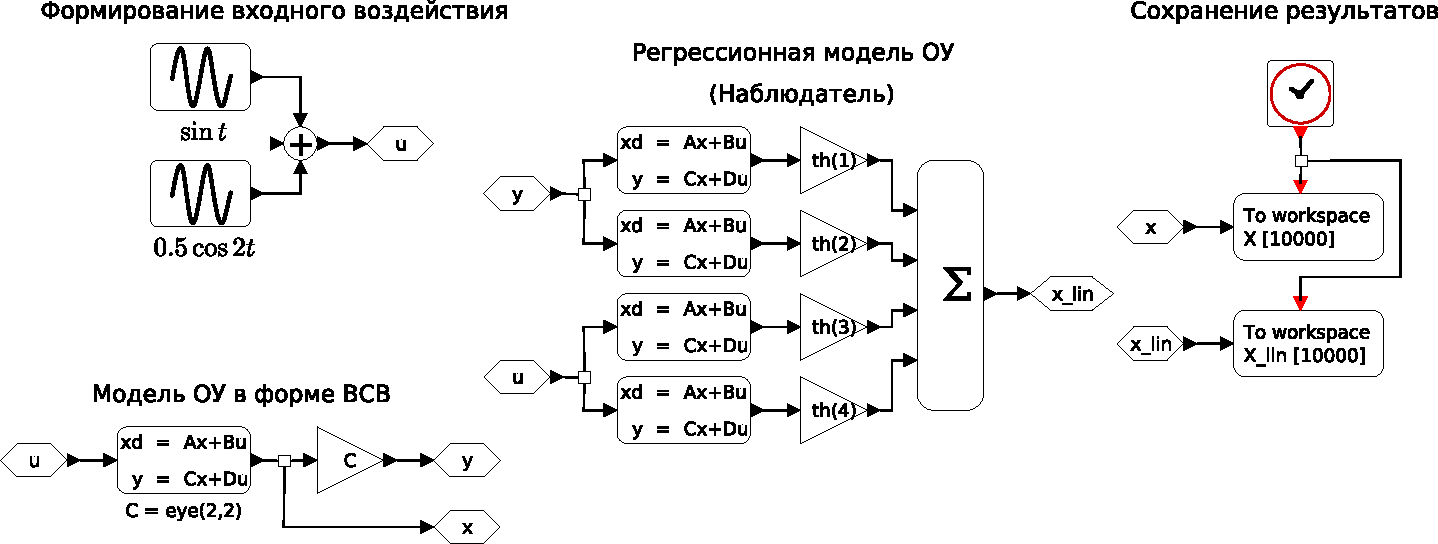
\includegraphics[width=\textwidth]{for_state.pdf}
    \caption{Схема моделирования, применяемая для проверки работы регрессионной модели.}
    \label{img_for_state}
\end{figure}

\begin{figure}[p]
    \centering
    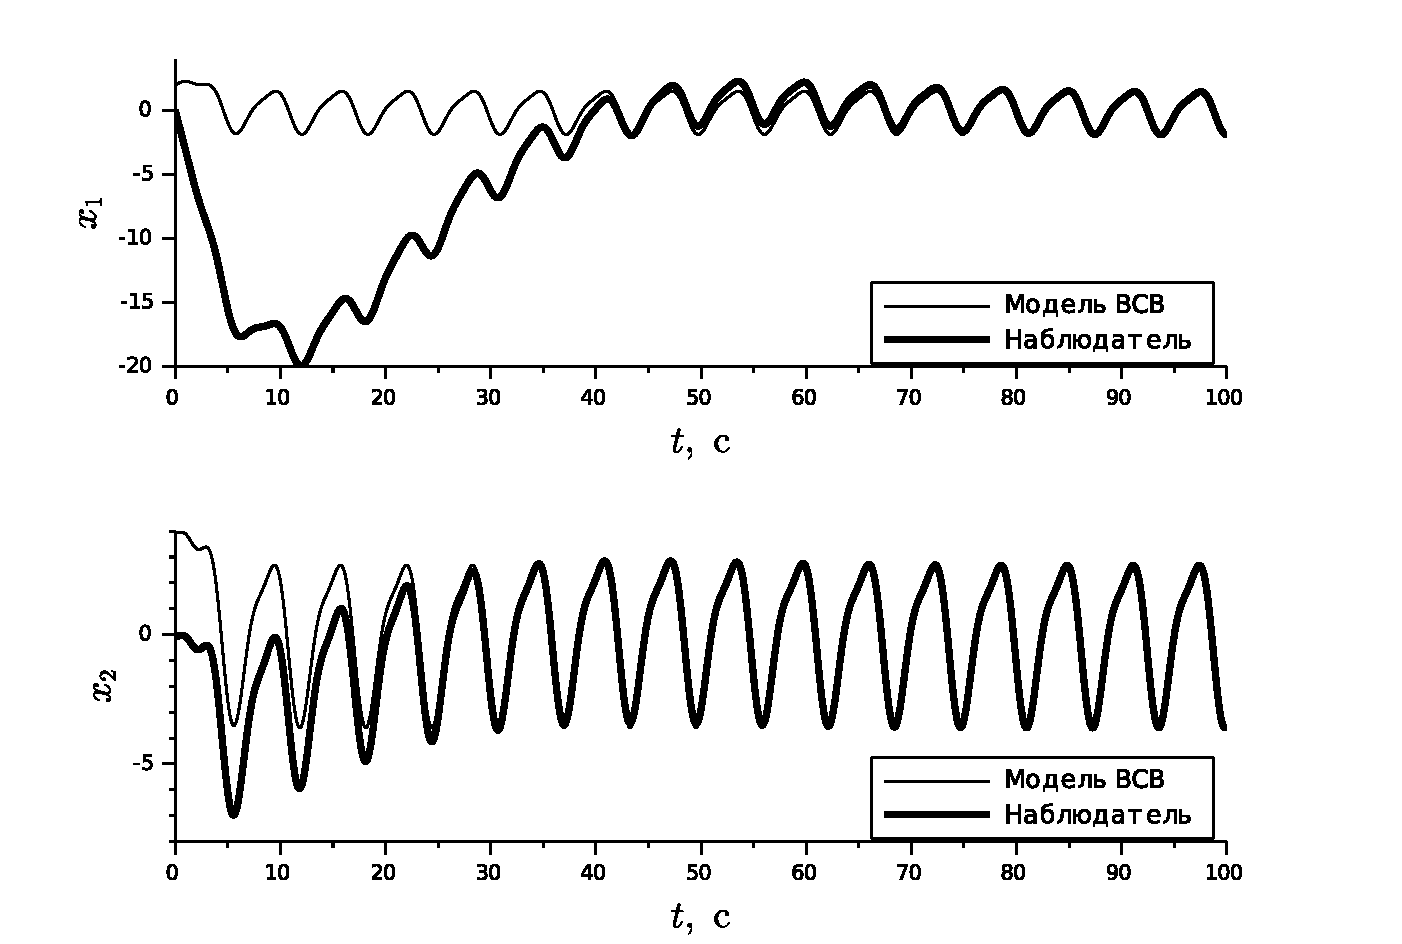
\includegraphics[width=\textwidth]{state_graphs.pdf}
    \caption{Графики выходных сигналов моделей ОУ при $x_1(0)=2$ и $x_2(0)=4$.}
    \label{img_state_graphs}
\end{figure}


\section{Выводы по работе}
В~результате проделанной работы для заданного объекта управления были построены его параметризованные представления относительно выходной переменной и вектора состояния.
Обе регрессионные модели оказались способными в точности воспроизводить происходящие в объекте движения спустя некоторое время, требующееся для протекания в них некоторых переходных процессов (см.~рисунки~\ref{img_output_graphs} и~\ref{img_state_graphs}).